\documentclass[conference]{IEEEtran}
\usepackage[utf8]{inputenc}

\usepackage{graphicx}
\usepackage[cmex10]{amsmath}
\usepackage{fixltx2e}

%%%%%%%%%%%%%%%%%%%%%%%%%%%%%%%%%%%%%%%%
%% some additions macros and packages that need to be included
\usepackage{xcolor}
\newcommand{\todo}[1]{{\color{red}[#1]}}
\newcommand{\new}[1]{\todo{NEW}}
\newcommand{\tocite}[1]{\todo{CITE #1}}
\newcommand{\psup}[1]{\ensuremath{^{(#1)}}}
\newcommand{\psupt}{\psup{t}}
%%%%%%%%%%%%%%%%%%%%%%%%%%%%%%%%%%%%%%%%


\usepackage{Sweave}
\begin{document}

\title{Some theoretical and experimental observerations on naïve discriminative learning}
\author{\IEEEauthorblockN{Stefan Evert}
\IEEEauthorblockA{Friedrich-Alexander-Universität Erlangen-Nürnberg\\
Email: stefan.evert@fau.de}
\and
\IEEEauthorblockN{Antti Arppe}
\IEEEauthorblockA{University of Alberta\\
Email: arppe@ualberta.ca}}

\maketitle

%\begin{abstract}
%The abstract goes here.
%\end{abstract}

% \IEEEpeerreviewmaketitle

\section{Introduction}
\label{sec:intro}

Natural language use is full of choices among multiple possible alternatives, whether phones, words, or constructions, which are influenced by a large number of contextual factors, and which rather exhibit asymptotic, imperfect tendencies favoring one or more of the alternatives, instead of single, categorical, perfect choices. This contrasts with item-by-item learning in simple controlled experiments which typically have been modelled by the Rescorla-Wagner equations \cite{rescorlawagner1972}. We find the former ``messy'' types of problems to be a key area of interest in modelling and understanding language use, and consequently consider the application of the Rescorla-Wagner equations -- in the form of a Naïve Discriminative Learning classifier -- to such complex phenomena of considerable utility in linguistic research. 
  
Naïve Discrimative Learning (NDL) \cite{baayenetal2011, baayen2011}, as implemented by Arppe et al.\ \cite{shaoul2014}, performs linguistic classification on the basis of direct associations between cues and outcomes, which are learned incrementally according to the Rescorla-Wagner (R-W) equations \cite{rescorlawagner1972, milleretal1995}.

Danks \cite{danks2003} argued that if the R-W equations successfully acquire the true associations between cues and outcomes, they should approximate an equilibrium state in which the expected change in association values is zero if a cue-outcome event is randomly presented to the learner.  This equilibrium state can be computed directly by solving a matrix equation, without carrying out many iterations of R-W updates, making NDL attractive as an efficient learning technique for quantitative investigations in linguistics.  The use of the Danks equilibrium also circumvents the problem that a simulation of an R-W learner does not truly converge to a single state unless the learning rate is gradually decreased. 

It is well known that the R-W equations are related to neural networks (through the ``delta rule'' for gradient-descent training of a single-layer perceptron) and to linear least-squares regression (e.g.\ \cite{gluckbower1988,danks2003,baayenetal2011}). Furthermore, empirical observations have shown that, compared to other statistical classification techniques (such as support vector machines, random forests, or memory-based learning), NDL appears to be most similar to logistic regression with respect to overall prediction accuracy, agreement among individual predicted outcomes, and the distribution of estimated probabilities \cite{arppebaayen2011}. However, many authors do not seem to be aware of the true depth of these similarities and of their implications.

While precise results on the correspondence of the \mbox{R-W} equations with a certain single-layer perceptron \cite[p.\ 155f]{suttonbarto1981} and with least-squares regression \cite[p.\ 457]{stone1986} are available, they are scattered across various publications, presented in different notations, and often stated without a full, self-contained derivation.  The most comprehensive treatment of the relation between R-W and various types of neural networks is a recent monograph by Dawson \cite{dawson2008}.  Dawson combines a mathematical comparison with various simulation experiments, but he rejects neural networks with a linear activation function as inappropriate \cite[p.\ 11]{dawson2008} and consequently does not discuss the connection to least-squares regression at all.  

In this paper, we collect and explain the precise equivalences between the R-W model, neural networks, and least-squares regression, using a consistent notation and giving mathematical derivations where appropriate.  In Sec.~\ref{sec:math-def} we present different forms of the R-W equations, including the stochastic version implicitly used by \cite{danks2003}. We then show that R-W is identical to gradient-descent training of a single-layer feed-forward neural network, which we refer to as a single layer perceptron (SLP)\footnote{The term SLP is often reserved for a particular form of such a single-layer network using a Heaviside activation function.  Here, we use it more generally to refer to any single-layer feed-forward network.} here (Sec.~\ref{sec:slp}). Based on this result, we give a new, simpler derivation of the equilibrium conditions of \cite{danks2003} and prove that they correspond to the solution of a linear least-squares regression problem (Sec.~\ref{sec:regression}). Sec.~\ref{sec:logistic} briefly addresses the similarity between R-W and logistic regression.  Finally we discuss some consequences of these new insights in Sec.~\ref{sec:consequence} and complement them with preliminary simulation experiments.

\section{The Rescorla-Wagner equations}
\label{sec:math-def}

This section gives a mathematically precise definition of the R-W model, following the notation of \cite{danks2003}.  The purpose of the R-W equations is to determine associations between a set of cues $C_1, \ldots, C_n$ and a single outcome $O$ in a population of event tokens $(\mathbf{c}\psupt, o\psupt)$, where $\mathbf{c}\psupt = (c_1\psupt, \ldots, c_n\psupt)$ is a vector of cue indicators for the event $t$ and $o\psupt$ an indicator for the outcome $O$.  Formally,
\begin{align}
  \label{eq:def-c-o}
  c_i\psupt &= 
  \begin{cases}
    1 & \text{if $C_i$ is present} \\
    0 & \text{otherwise}
  \end{cases}
  &
  o\psupt &= 
  \begin{cases}
    1 & \text{if $O$ results} \\
    0 & \text{otherwise}
  \end{cases}
\end{align}
for $t = 1, \ldots, m$ (and $m = \infty$ can be allowed).  We assume that one of the cues is a ``background stimulus'' that is always present, e.g.\ $c_1\psupt \equiv 1$.  This is necessary in order to obtain full equivalence with least-squares regression.  It is also intuitively plausible: without the background stimulus, the learner would not be able to expect the outcome $O$ in the absence of any explicit cues. 

When presented with an event $(\mathbf{c}, o)$, the R-W equations update the associations $V_i$ between the individual cues and the outcome according to Eq.~(\ref{eq:def-rw}), which is a more formal notation of Eq.~(1) from \cite[p.\ 111]{danks2003}.
\begin{equation}
  \label{eq:def-rw}
  \Delta V_i =
  \begin{cases}
    0 & \text{if } c_i = 0\\
    \alpha_i \beta_1 \bigl(\lambda - \sum_{j=1}^n c_j V_j \bigr) & \text{if } c_i = 1 \wedge o = 1 \\
    \alpha_i \beta_2 \bigl(0 - \sum_{j=1}^n c_j V_j \bigr) & \text{if } c_i = 1 \wedge o = 0
  \end{cases}
\end{equation}
Here, $\alpha_i$ is a measure of the salience of cue $C_i$, $\beta_1$ and $\beta_2$ are learning rates for positive ($o=1$) and negative ($o=0$) events, and $\lambda$ is the maximal activation level of the outcome $O$.  A simplified form of the R-W equations proposed in the context of artificial neural networks \cite{widrowhoff1960} assumes that $\alpha_1 = \dots = \alpha_n = 1$,  $\beta_1 = \beta_2 = \beta$ and $\lambda = 1$ (known as the Widrow-Hoff or W-H rule).

We will make the assumption that $\beta_1 = \beta_2 = \beta$ from here on, but put no restrictions on $\alpha_i$ or $\lambda$.  The R-W equations can then be combined into a single formula
%%
\begin{equation}
  \label{eq:rw-single}
  \Delta V_i = c_i \alpha_i \beta \left( \lambda o - \sum_{j=1}^n c_j V_j \right) .
\end{equation}
%%
In linguistics, NDL is often used to model a natural learning process, where event tokens are randomly sampled from the population, rather than a controlled experimental procedure.  In this case, there is little point in studying the associations acquired by one particular learner after a given number of training events, i.e.\ the sequence of association vectors $\mathbf{V}\psupt = (V_1\psupt, \ldots, V_n\psupt)$.  We are rather interested in the typical associations obtained by averaging across a large number of learners, i.e.\ the expected values $E[\mathbf{V}\psupt]$, and in how much variability there is between individual learners.  Correspondingly, the events $(\mathbf{c}\psupt, o\psupt)$ are interpreted as i.i.d.\ random variables sampled from the population of event tokens.  As will be shown in the following section, we can use theoretical arguments to determine the asymptotic behaviour $\lim_{t\to \infty} E[\mathbf{V}\psupt]$ of R-W learning, and we can carry out simulation experiments in order to study variability between learners.

Since the event $(\mathbf{c}\psupt, o\psupt)$ at time $t$ is independent from the current associations $\mathbf{V}\psupt$, we can take expectations on both sides of Eq.~(\ref{eq:rw-single}) to obtain $E[\mathbf{V}\psup{t+1}] = E[\mathbf{V}\psupt] + E[\Delta \mathbf{V}\psupt]$ with
%%
\begin{equation}
  \label{eq:exp-rw}
  \begin{split}
    E[\Delta V_i\psupt]
    &= \alpha_i\beta \left( \lambda E[o c_i] - \sum_{j=1}^n E[c_i c_j] E[V_j\psupt] \right) \\
    &= \alpha_i\beta \left( \lambda P(O, C_i) - \sum_{j=1}^n P(C_i, C_j) E[V_j\psupt] \right) .
  \end{split}
\end{equation}
%% 
Note that $E[c_i c_j V_j] = E[c_i c_j]\cdot E[V_j]$ because the random variable $V_j$ is independent from the $c_i$ and $c_j$, that the expectation of the product $o c_i$ of two indicator variables is the co-occurrence probability of the two events, i.e.\ $E[o c_i] = P(O, C_i)$, and that $E[c_i c_j] = P(C_i, C_j)$ for the same reason.  Eq.~(\ref{eq:exp-rw}) is identical to \cite[Eq.~(A-5)]{gluckbower1988} except for differences in notation.

Danks \cite{danks2003} argued that a successful R-W learner should converge to an equilibrium state $\mathbf{V} = \lim_{t\to\infty} E[\mathbf{V}\psupt]$ of the expected association vector, where the expected update $E[\Delta \mathbf{V}] = 0$.  From Eq.~(\ref{eq:exp-rw}), we obtain the identity
\begin{equation}
  \label{eq:danks-equi}
  \lambda P(O, C_i) - \sum_{j=1}^n P(C_i, C_j) V_j = 0
\end{equation}
for the Danks equilibrium, which is equal to his Eq.~(11) \cite[p.\ 113]{danks2003} multiplied by $P(C_i)$.

\section{R-W and the single layer perceptron}
\label{sec:slp}

We will now formulate a single-layer feed-forward neural network (SLP) whose learning behaviour -- with gradient-descent training, which corresponds to the backprop algorithm for a SLP and is also known as the ``delta rule'' in this case -- is identical to the R-W equations with equal positive and negative learning rates $\beta_1 = \beta_2$ (but no other restrictions).  The SLP requires a slightly different representation of events as pairs $(\mathbf{x}\psupt, z\psupt)$ with
\begin{align}
  \label{eq:def-x-z}
  x_i\psupt &= 
  \begin{cases}
    a_i & \text{if $C_i$ is present} \\
    0 & \text{otherwise}
  \end{cases}
  &
  z\psupt &= 
  \begin{cases}
    \lambda & \text{if $O$ results} \\
    0 & \text{otherwise}
  \end{cases}
\end{align} 
Here, $a_i > 0$ is a (different) measure of the salience of cue $C_i$ and $\lambda > 0$ the maximum activation of outcome $O$.  Note that the event representation $(\mathbf{x}, z)$ is connected to the representation $(\mathbf{c}, o)$ through the equivalences $x_i = a_i c_i$ and $z = \lambda o$.  In the simplified W-H case, the two representations are identical.

The SLP computes the activation of the outcome as a linear combination $y = \sum_{i=1}^n w_i x_i$ of the input variables, where $\mathbf{w} = (w_1, \ldots, w_n)$ is the weight vector of the network.  It uses a linear activation function $h(y) = y$ and a Euclidean cost function for the difference between $y$ and the desired activation level $z$.  The cost associated with a given event token $(\mathbf{x}, z)$ is thus
\begin{equation}
  \label{eq:cost-single}
  E(\mathbf{w}, \mathbf{x}, z) = (z - y)^2 = \biggl( z - \sum_{i=1}^n w_i x_i \biggr)^2 .
\end{equation}
For batch updates based on the full population of event tokens, the corresponding batch cost is
\begin{equation}
  \label{eq:cost-batch}
  E(\mathbf{w}) = \sum_{t=1}^m E(\mathbf{w}, \mathbf{x}\psupt, z\psupt) .
\end{equation}
If smaller batches are used, the sum $j$ ranges over a subset of the population for each update step, or a single token in the extreme case of item-by-item learning.

Presented with a single event token $(\mathbf{x}, z)$, gradient-descent training of the SLP updates the weight vector by 
\begin{equation}
  \label{eq:gd-rule}
  \Delta w_i = -\delta \frac{\partial E(\mathbf{w}, \mathbf{x}, z)}{\partial w_i}
\end{equation}
where $\delta > 0$ is the learning rate and the gradient $\partial E / \partial w_i$ is given by
\begin{equation}
  \label{eq:gd-gradient}
  \frac{\partial E(\mathbf{w}, \mathbf{x}, z)}{\partial w_i} = 2 (z - y) (-x_i)
  = -2 \biggl( z - \sum_{j=1}^n w_j x_j \biggr) x_i .
\end{equation}
%%
Inserting the equalities $x_i = a_i c_i$ and $z = \lambda o$, we obtain
\begin{equation}
  \label{eq:slp-delta}
  \Delta w_i =
  \begin{cases}
    0 & \text{if } c_i = 0\\
    2 \delta a_i \bigl(\lambda - \sum_{j=1}^n c_j a_j w_j \bigr) & \text{if } c_i = 1 \wedge o = 1 \\
    2 \delta a_i \bigl(0 - \sum_{j=1}^n c_j a_j w_j \bigr) & \text{if } c_i = 1 \wedge o = 0 
  \end{cases}
\end{equation}
Comparing this with Eq.~(\ref{eq:def-rw}), we can set $V_j = a_j w_j$, i.e.\ we interpret the weight vector $\mathbf{w}$ of the SLP as salience-adjusted cue-outcome associations.  With $\Delta V_i = a_i \Delta w_i$, we obtain
\begin{equation}
  \label{eq:slp-delta-as-rw}
  \Delta V_i =
  \begin{cases}
    0 & \text{if } c_i = 0\\
    2 \delta a_i^2 \bigl(\lambda - \sum_{j=1}^n c_j V_j \bigr) & \text{if } c_i = 1 \wedge o = 1 \\
    2 \delta a_i^2 \bigl(0 - \sum_{j=1}^n c_j V_j \bigr) & \text{if } c_i = 1 \wedge o = 0
  \end{cases}
\end{equation}
which is identical to the R-W equations for $\beta_1 = \beta_2 = 2\delta$ and $\alpha_i = a_i^2$.

The assumption $\beta_1 = \beta_2$ can be relaxed if we change the representation of events to
\begin{equation}
  \label{eq:def-x-mod}
  x_i\psupt = 
  \begin{cases}
    a_i & \text{if } c_i = 1 \wedge o = 1 \\
    a_i \sqrt{\frac{\beta_2}{\beta_1}} & \text{if } c_i = 1 \wedge o = 0 \\
    0 & \text{otherwise}
  \end{cases}
\end{equation}
i.e.\ if we allow the salience of cues to differ between positive ($o = 1$) and negative ($o = 0$) events; the scaling factor $\beta_2 / \beta_1$ is the same for all cues $C_i$.  We do not pursue this extension further here because -- unlike other parameters of R-W -- the ratio between positive and negative learning rates has a complex effect on the equilibrium state.  As \cite{danks2003} has already observed, neither the cue saliences $\alpha_i$ nor the overall learning rate $\beta = \beta_1 = \beta_2$ affect the equilibrium and the maximum activation level $\lambda$ merely results in a linear scaling. 

\section{R-W and least-squares regression}
\label{sec:regression}

We have shown in Sec.~\ref{sec:slp} that the R-W equations describe the gradient-descent training of a SLP for the linear regression problem
\begin{equation}
  \label{eq:lsr-def}
  \min_{\mathbf{w}} E(\mathbf{w})
  = \min_{\mathbf{w}} \sum_{t=1}^m E(\mathbf{w}, \mathbf{x}\psupt, z\psupt) .
\end{equation}
This equivalence holds generally, not only in the case of the simplified W-H rule.  Thus, both R-W and our SLP aim to solve the same least-squares regression.

If the training procedure is successful, the weight vector $\mathbf{w}$ should approach the least-squares solution of the regression problem.  With item-by-time updates (corresponding to the behaviour of a single R-W learner), convergence cannot be achieved unless the learning rate is gradually reduced.\footnote{In fact, item-by-item updates do converge if the regression problem is linearly separable, i.e.\ if perfect predictions can be achieved. This situation is highly unlikely in linguistic applications of NDL, though.}  With batch updates based on the entire population of event tokens, the cost $E(\mathbf{w})$ is a convex function of $\mathbf{w}$ and the gradient descent procedure converges to its unique minimum after a sufficient number of iterations.\footnote{In fact, the minimum of $E(\mathbf{w})$ might not be unique under certain circumstances, viz. if the correlation matrix of the cues is not positive definite; cf. \cite[pp.\ 115--116]{danks2003} for the special case of ``coextensive'' cues. In order to keep the discussion straightforward, we assume the general case of a unique minimum in the present paper.}
Since batch updates compute the average of Eq.~(\ref{eq:slp-delta-as-rw}) over all event tokens, they correspond to R-W updates for the expected associations $E[\mathbf{V}\psupt]$ according to Eq.~(\ref{eq:exp-rw}).


In order to express Eq.~(\ref{eq:lsr-def}) more concisely, we define an $m\times n$ matrix $\mathbf{X} = (x_i\psupt) = (x_{ti})$ of cues for all event tokens in the population.  The rows of this matrix correspond to event tokens $t$, the columns to cues $i$; i.e.\ row number $t$ contains the input vector $\mathbf{x}\psupt$.  The particular ordering of the event tokens is irrelevant.  We also define the column vector $\mathbf{z} = (z\psup{1}, \ldots, z\psup{m}) = (z_1, \ldots, z_m)$ of outcomes and recall that $\mathbf{w} = (w_1, \ldots, w_n)$ is a column vector of SLP weights.  The batch cost can now be written as a dot product
\begin{equation}
  \label{eq:lsr-matrix}
  E(\mathbf{w}) = \bigl( \mathbf{z} - \mathbf{X} \mathbf{w} \bigr)^T \bigl( \mathbf{z} - \mathbf{X} \mathbf{w} \bigr) .
\end{equation}
The least-squares solution must satisfy the condition $\nabla E(\mathbf{w}) = \mathbf{0}$, which leads to the so-called normal equations \cite[p.\ 142]{bishop2006}
\begin{equation}
  \label{eq:lsr-normal}
  \mathbf{X}^T \mathbf{X} \mathbf{w} = \mathbf{X}^T \mathbf{z} .
\end{equation}
In the case of the W-H rule, $\mathbf{X}$ is a coincidence matrix between cues and events, with $x_{ti} \in \{0, 1\}$, and $\mathbf{z}$ is a vector of indicator variables $z_t \in \{0, 1\}$.  A straightforward calculation shows that $\mathbf{X}^T \mathbf{X}$ is a square matrix of co-occurrence counts between cues:
\[
(\mathbf{X}^T \mathbf{X})_{ij} = \sum_{t=1}^m x_{ti} x_{tj} = f(C_i, C_j) .
\]
Similarly, $\mathbf{X}^T \mathbf{z}$ is a vector of co-occurrence counts between the cues and the outcome $O$:
\[
(\mathbf{X}^T \mathbf{z})_i = \sum_{t=1}^m x_{ti} z_t = f(C_i, O) .
\]
Dividing Eq.~(\ref{eq:lsr-normal}) by $m$, we obtain Eq.~(\ref{eq:danks-equi}) with $\lambda = 1$, i.e.
\[
P(O, C_i) - \sum_{j=1}^n P(C_i, C_j) V_j = 0
\]
which is the same as Danks's Eq.~(3) \cite[p.\ 112]{danks2003} with rows multiplied by $P(C_i)$.  Since linear regression is invariant wrt.\ the salience factors $a_i$ (the weights are simply adjusted by reciprocal factors $1 / a_i$ to achieve the same regression predictions) and scales linearly with $\lambda$, equivalence to the equilibrium conditions \cite[pp.\ 112--114]{danks2003} also holds for arbitrary values of $a_i$ and $\lambda$.

In the general case where the regression problem has a unique solution, $\mathbf{X}^T \mathbf{X}$ is symmetric and positive definite.  It can therefore be inverted and the least-squares solution is given by
\begin{equation}
  \label{eq:lsr-solution}
  \mathbf{w}^* = (\mathbf{X}^T \mathbf{X})^{-1} \mathbf{X}^T \mathbf{z} .
\end{equation}
Standard statistical software such as R \cite{R2015} can be used to compute $\mathbf{w}^*$ reliably and efficiently.
This least-squares solution corresponds to the equilibrium state $\mathbf{V} = \lim_{t\to\infty} E[\mathbf{V}\psupt]$ of the R-W learner.  If we are mainly interested in such an asymptotic equilibrium,
it is not necessary to carry out the iterative training procedure of the R-W model or the neural network, and there is no need to worry about convergence of the training.


\section{R-W and logistic regression}
\label{sec:logistic}

If the goal of an NDL application is to make a probabilistic prediction about the outcome $O$ based on cues $C_i$, most machine-learning textbooks would recommend logistic regression \cite[p.\ 205]{bishop2006} instead of a least-squares approach.  Logistic regression can be understood as a SLP with logistic activation function
%%
\begin{equation}
  \label{eq:logistic-function}
  h(y) = \frac{1}{1 + e^{-y}}
\end{equation}
%%
and $y = \sum_{i=1}^n w_i x_i$.  Since $0\leq h(y)\leq 1$, it can be interpreted as the predicted probability of the outcome $O$ (i.e.\ of $o=1$) given the cues $x_1, \ldots, x_n$.  The accuracy of a prediction is assessed by the Bernoulli cost
%%
\begin{equation}
  \label{eq:bernoulli-cost}
  \begin{split}
    E(\mathbf{w}, \mathbf{x}, o) 
    &= \begin{cases}
      -\log h(y) & \text{if } o = 1 \\
      -\log (1 - h(y)) & \text{if } o = 0
    \end{cases}
    \\
    &= - o \log h(y) - (1-o) \log (1 - h(y))
  \end{split}
\end{equation}
%%
which indicates how well the SLP was able to predict the presence or absence of the outcome.  Item-by-item gradient-descent training leads to updates of the form
%%
\begin{equation}
  \label{eq:lrm-gd}
  \Delta w_i = -\delta \frac{\partial E(\mathbf{w}, \mathbf{x}, o)}{\partial w_i}
\end{equation}
%%
with 
%%
\begin{equation}
  \label{eq:lrm-gd-gradient}
  \frac{\partial E(\mathbf{w}, \mathbf{x}, o)}{\partial w_i}
  = (h(y) - o) x_i 
\end{equation}
%%
according to \cite[p.\ 205]{bishop2006}.  Interpreting the weights $w_i$ as salience-adjusted associations $V_j = a_j w_j$ as in Sec.~\ref{sec:slp} and keeping in mind that $x_i = a_i c_i$, we obtain a form that is strikingly similar to the R-W equations.
%%
\begin{equation}
  \label{eq:lrm-rw}
  \Delta V_i =
  \begin{cases}
    0 & \text{if } c_i = 0\\
    \delta a_i \left( 1 - h \bigl( \sum_{j=1}^n c_j V_j \bigr) \right) & \text{if } c_i = 1 \wedge o = 1 \\
    \delta a_i \left( 0 - h \bigl( \sum_{j=1}^n c_j V_j \bigr) \right) & \text{if } c_i = 1 \wedge o = 0
  \end{cases}
\end{equation}
%%
The only difference from Eq.~(\ref{eq:def-rw}) is that the total association computed by the learner is now transformed into a probability by the logistic activation function $h(y)$.

Therefore, it would be particularly interesting to observe the behavior of such a logistic regression learner and compare it in detail with an NDL learner based on the R-W equations, using both synthetic data sets and real linguistic data. General rules-of-thumb for logistic regression recommend at least 10 or 20 times as many datapoints as there are variables (i.e.\ cue-outcome pairings) in order to gain a valid and reliable model (e.g. \cite{peduzzi1996}; \cite[p.\ 116]{arppe2008}). The same recommendation is usually given for linear regression in order to avoid overfitting, but there is one important difference between the two approaches. If the number of cues is sufficiently large, the learning problem becomes separable and the system can in principle make perfect predictions. In this case, the weights $\mathbf{w}$ of the logistic regression learner will diverge in an attempt to predict a probability of $p=1$ ($w_i \to \infty$) or $p=0$ ($w_i\to -\infty$). NDL, on the other hand, will easily reach the perfect solution as an equilibrium point, with well-behaved and interpretable cue-outcome association strengths $\mathbf{V}$. Experimental evidence found by Arppe and Baayen \cite{arppebaayen2011} corroborates this analysis.


\section{Consequences}
\label{sec:consequence}


\begin{figure}[!t]
\centering
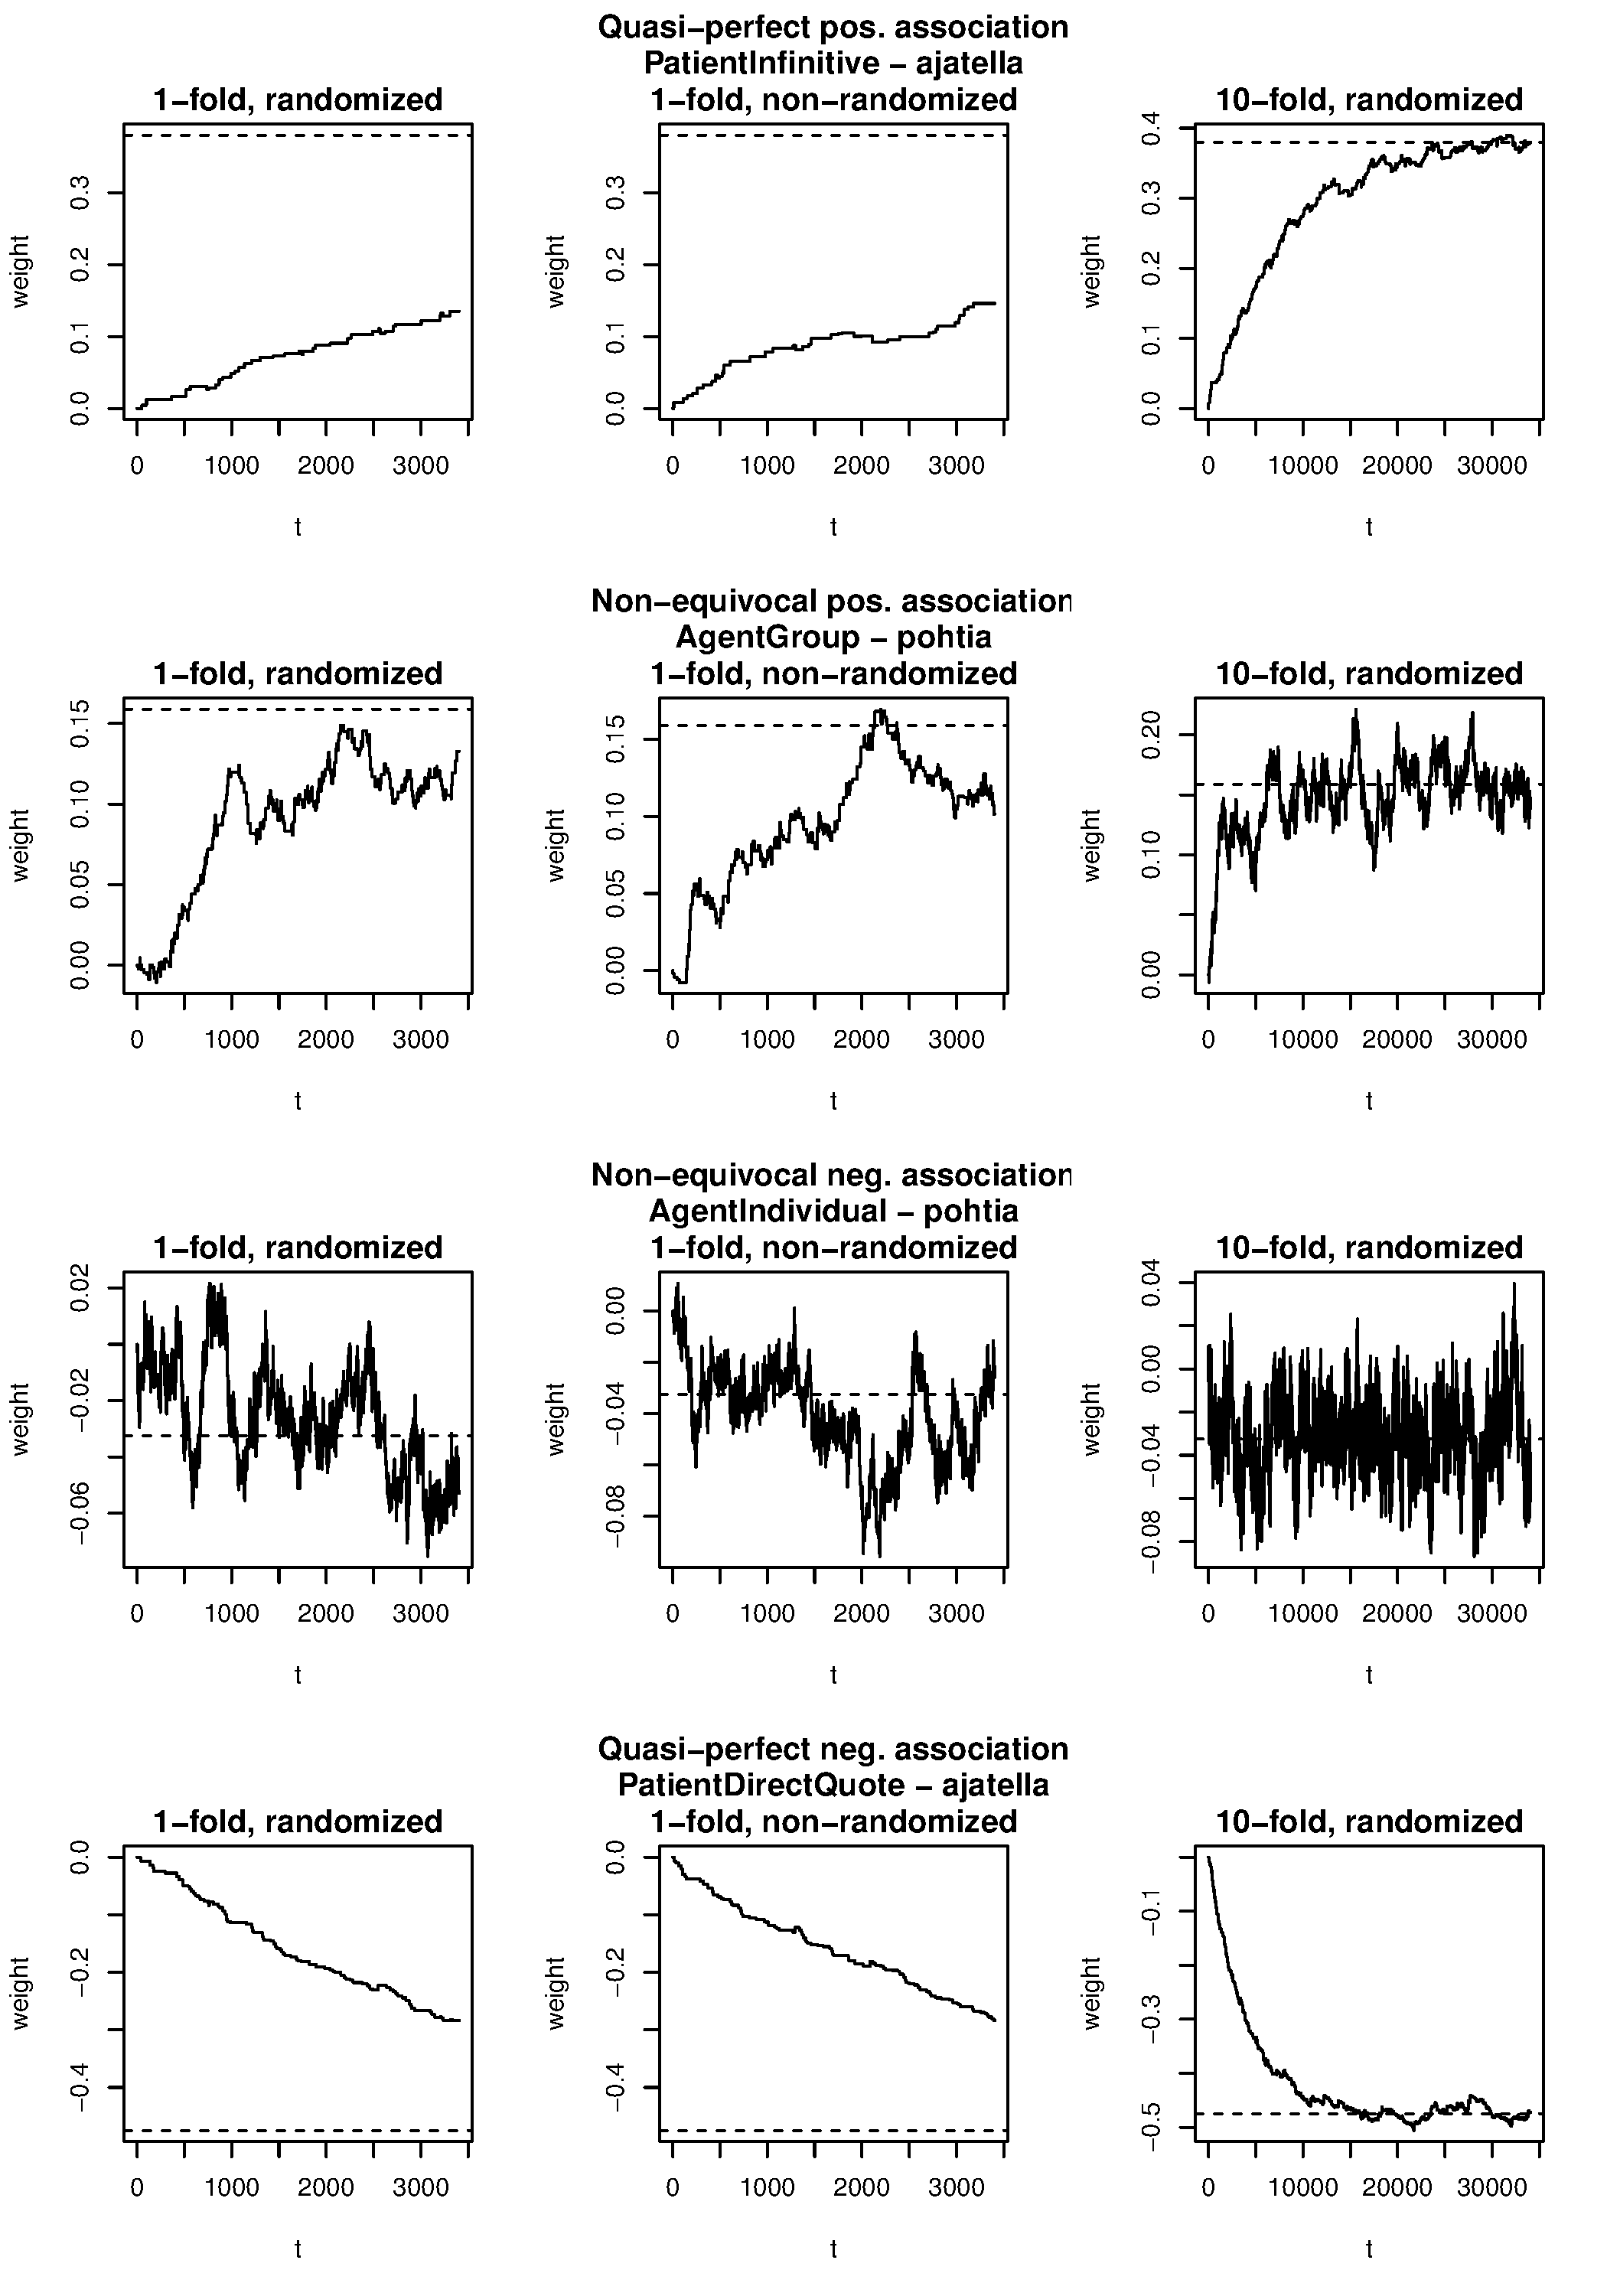
\includegraphics[width=2.5in]{QITL6_abstract_final-think_conv.png}
\caption{Simulation results for a Finnish \textsc{think} dataset with selected linguistic contextual features (cues) and verbs (outcomes), using (i) R-W learning within a randomized version of the original dataset (3404 datapoints) (ii) R-W learning with a non-randomized version of the dataset (3404 datapoints), and (iii) R-W learning with a 10-fold, randomized multiple of the dataset (altogether 34040 datapoints). R-W cue-outcome association values shown as a solid line; corresponding equilibrium association values as a dotted line.}
\label{think_weights}
\end{figure}



\begin{figure}[!t]
\centering
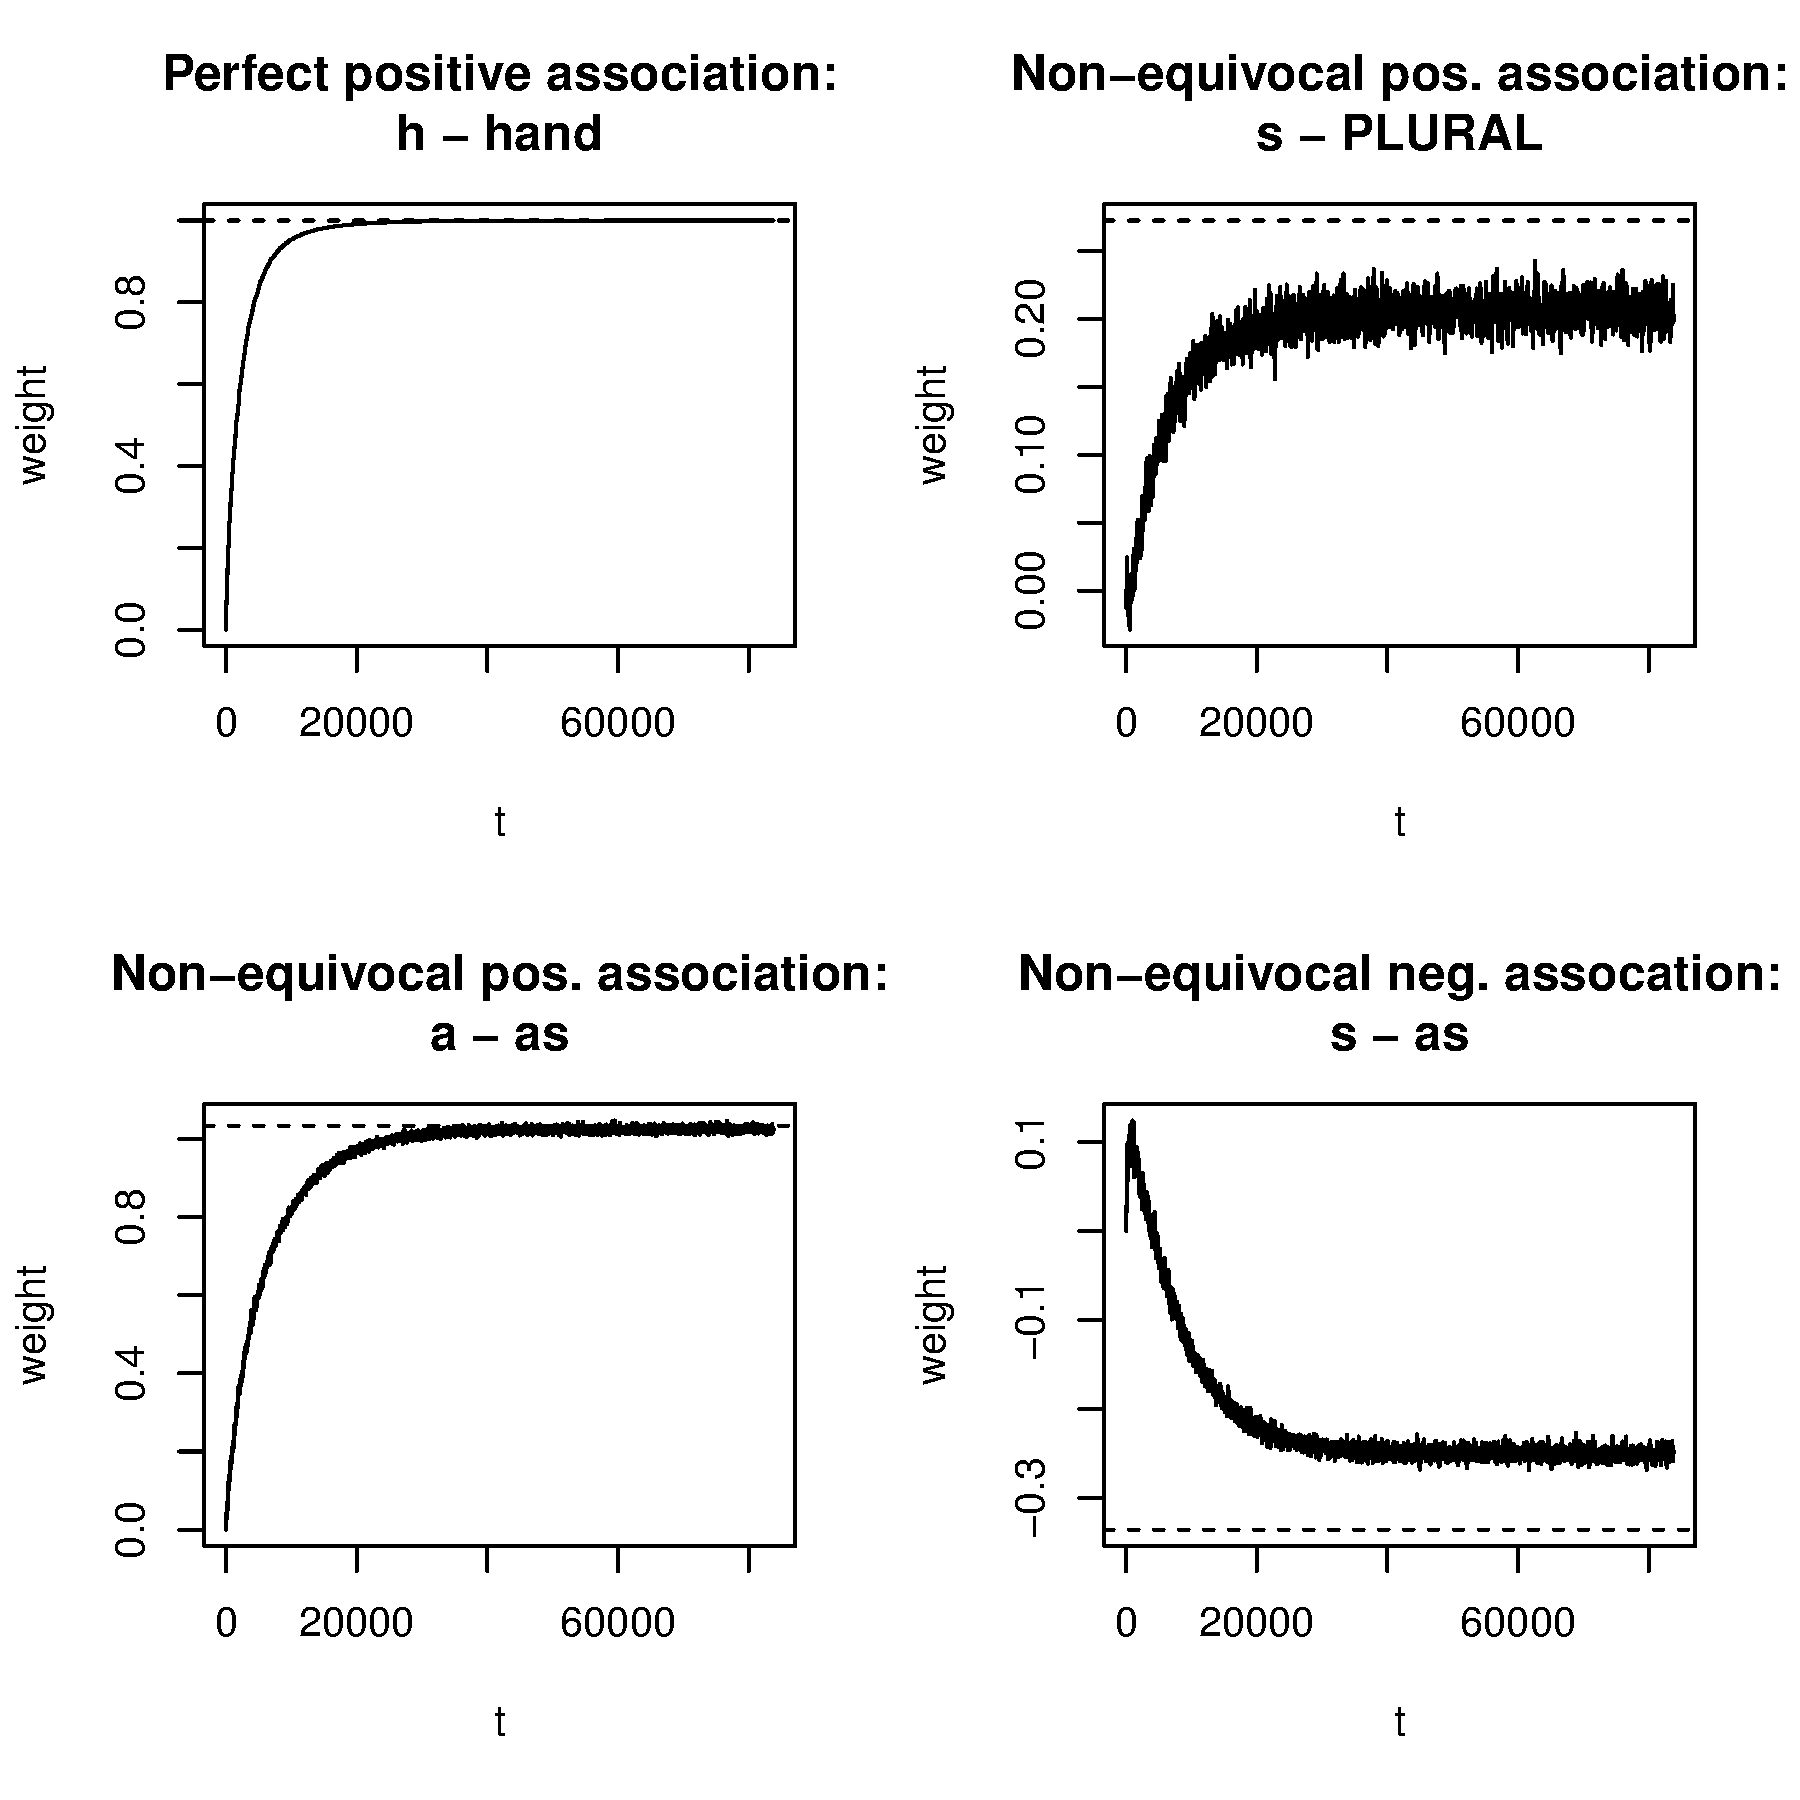
\includegraphics[width=2.5in]{QITL6_abstract_final-plurals_conv.png}
\caption{Simulation results for a tiny, artificial dataset of English nouns and their pluralizations (10 types with 419 tokes), with selected orthographical unigraph features (cues) and lemmas (outcomes), using R-W learning with a 200-fold, randomized version of the dataset \cite[Extension of Fig.~4]{baayenetal2011}. R-W cue-outcome association values shown as a solid line; corresponding equilibrium association values as a dotted line. N.B. In the underlying representation of cues and outcomes in this example, and the subsequent calculations of their incremental R-W associations weights, multiple occurrences of the same cue within the same event, i.e. \textit{s} in \textit{lass}, are encoded as distinct cues (cf. the manual page for the \texttt{plurals} dataset in the \texttt{ndl} package \cite{shaoul2014}).}
\label{plural_weights}
\end{figure}


\begin{figure}[!t]
\centering
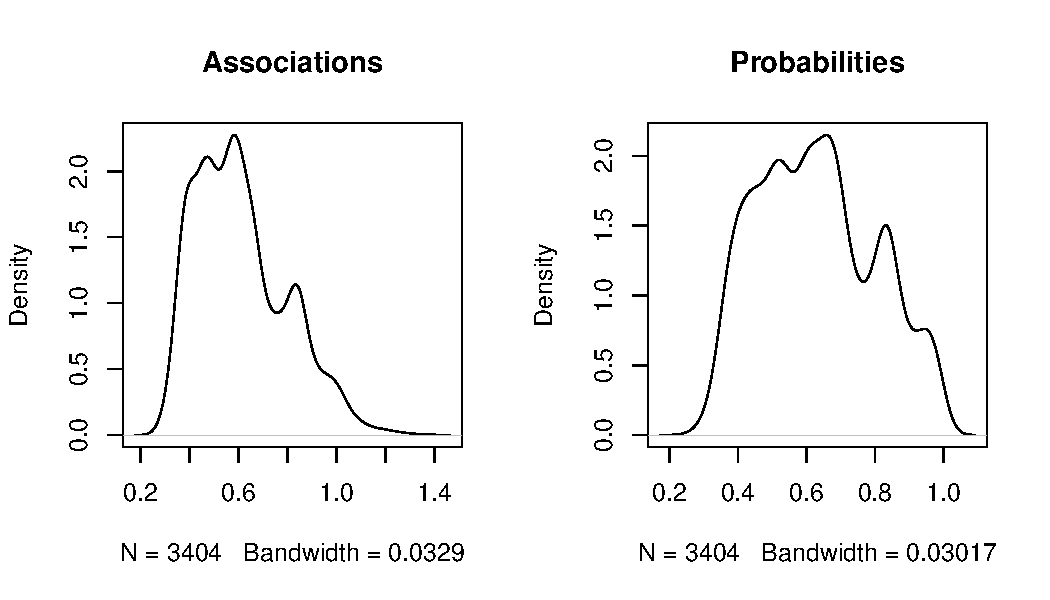
\includegraphics[width=2.5in]{QITL6_abstract_final-think_assocs_probs.pdf}
\caption{Distributions of instance-wise estimated maximal associations (NDL) and probabilities (GLM) using the Finnish \textsc{think} dataset ($n=3404$).}
\label{think_assocs_probs}
\end{figure}

We have shown that R-W association learning, a linear SLP neural network and linear regression are fully equivalent and should ideally lead to the same least-squares solution.  As long as a researcher is only interested in the final result of associative learning, not in the iterative process itself, it is sufficient to calculate the least-squares solution directly from Eq.~(\ref{eq:lsr-solution}). Essentially, the R-W salience factors $\alpha_i$ have no effect on the learning result -- because linear regression is not sensitive to such a scaling of the input variables -- but only on the learning process: associations for cues with high salience $\alpha_i$ are learnt faster than for other cues.  The parameter $\lambda$ leads to a (trivial) linear scaling of the learning result, but has no effect on the learning process.  Only different learning rates $\beta_1\neq \beta_2$ affect the equilibrium solution, because they modify the matrix $\mathbf{X}^T \mathbf{X}$ in a non-trivial way.  Eq.~(\ref{eq:def-x-mod}) suggests that $\beta_1$ and $\beta_2$ can be understood as salience measures for positive and negative outcomes.  Changing the prevalence of positive and negative events in the population -- in proportion to $\beta_1$ and $\beta_2$ -- would have the same effect.

If R-W association learning or SLP training does not approximate the least-squares solution, it can arguably be considered to have failed.  The only research question of interest that requires R-W iteration or application of the delta rule is thus: Under which circumstances and for which parameter settings does the R-W iteration converge to or at least approximate the linear regression? This is particularly relevant for single-event updates (according to the R-W equations), which are much less robust and lead to larger fluctuations than batch updates.  We plan to study these issues with the help of simulation experiments.

For instance, with a real dataset on the relationship between 46 linguistic contextual features as cues and 3404 occurrences of 4 near-synonymous Finnish \textsc{think} verbs as outcomes \cite{arppe2008, arppe2013, shaoul2014}, the cue-outcome associations arising from a simulation of R-W learning (using the default parameters) do appear to converge to the equilibrium values eventually (\figurename~\ref{think_weights}). For the non-equivocal contextual features that occur, to a higher or lower degree, with multiple outcomes (e.g.\ \textsc{AgentGroup} and \textsc{AgentIndividual} with \emph{pohtia}), this convergence seems to happen early, well within the course of the dataset. In contrast, with near-categorical features that in practice occur with only one of the four outcomes (e.g.\ the near-categorical co-occurrence of \textsc{PatientInfinitive} with \emph{ajatella} vs.\ the categorical non-occurrence of \textsc{PatientDirectQuote} with this same verb), convergence appears to happen much slower, so that multiple iterations over the full data set (as many as five or more times) are needed to approximate the equilibrium state.  Furthermore, this simulation clearly shows, particularly in the case of \textsc{AgentIndividual} and \emph{pohtia}, a remaining, sometimes quite substantial oscillation in the cue-outcome associations weights. In this respect, establishing how the learning parameters $\beta_1$ and $\beta_2$ might be adjusted in the course of the R-W learning process would be worthwhile. Interestingly, for the quasi-perfect cases, it does not seem to have an effect on the asymptotic result of R-W learning whether the order of datapoints is randomized in the learning process or not, in contrast to reservations in \cite[p.\ 119]{danks2003} -- but for the non-equivocal cases, the assumption of randomized order appears motivated. Of course, in all this one generally presumes that the proportions of the cue-outcome co-occurrences are the same in the overall population from which the dataset has been sampled.

In contrast, using a tiny, artificial dataset for English nouns and their pluralizations (10 types with 419 tokes), with orthographical unigraph features as cues and lemmas or number as outcome \cite[Fig.~4]{baayenetal2011}, the cue-outcome association weights arising from R-W learning do not show signs of converging to the equilibrium values at all in some cases, even after 200 iterations over the randomized dataset, e.g.\ for `\emph{s}' as cue and \textsc{plural} as outcome, or `\emph{s}' as cue and `\emph{as}' as outcome (\figurename~\ref{plural_weights}).\footnote{Among various versions of the \texttt{ndl} package \cite[v0.1.6 vs.\ 0.2.16]{shaoul2014}, there are several variants as how to calculate the equilibrium weights, but that does not seem to be the source of the observed non-convergence. In this paper, we have used \texttt{ndl v0.1.6}.}

\section{Open questions and future work}
\label{sec:outlook}

Having established NDL as a form of linear least-squares regression, with its well-known drawbacks (e.g.\ a propensity for overfitting the training data, especially if there is a large number $n$ of cues), it will be interesting to contrast it with more state-of-the-art machine learning techniques, as a systematic follow-up and analysis of the empirical observations in \cite{arppebaayen2011}.\footnote{Results using the Finnish \textsc{think} dataset \cite{arppe2008, arppe2013} indicated that (i) outcomes predicted by NDL and GLM (in the case of a 4-way \emph{polytomous} outcome using the \emph{one-vs-rest} technique implemented in the R package \texttt{polytomous} \cite{arppe2013}) agree with a rate of 94.8\%; (ii) the distributions of instance-wise maximum NDL cumulative association weights and corresponding maximum GLM expected probabilities have similar general distribution contours (cf. \figurename ~\ref{think_assocs_probs}); (iii) instance-wise maximum NDL association weights and corresponding maximum GLM expected probabilities are highly correlated, with $r_{Spearman}=.950$; and (iv) the same holds for individual NDL association weights and GLM log-odds, with $r_{Spearman}=.897$.} Using real linguistic data sets, we plan to pursue further the mathematical analysis and empirical study of (i) logistic regression (a subtype of the Generalized Linear Model, GLM), which is considered more appropriate for categorical data than linear least-squares regression, and (ii) regularization techniques for logistic as well as linear regression, which control overfitting and encourage sparse solutions. Finally, as NDL through the R-W equations is based on a model of human learning, an interesting avenue for further research would be to compare cue-outcome associations weights (based on applying NDL to corpus data that represent naturally produced language) with experiments that would hone in on the cognitive processing of the same linguistic stimuli by human participants.

% use section* for acknowledgment
%\section*{Acknowledgment}
% The authors would like to thank...

% trigger a \newpage just before the given reference
% number - used to balance the columns on the last page
% adjust value as needed - may need to be readjusted if
% the document is modified later
%\IEEEtriggeratref{8}
% The "triggered" command can be changed if desired:
%\IEEEtriggercmd{\enlargethispage{-5in}}

% references section

% can use a bibliography generated by BibTeX as a .bbl file
% BibTeX documentation can be easily obtained at:
% http://www.ctan.org/tex-archive/biblio/bibtex/contrib/doc/
% The IEEEtran BibTeX style support page is at:
% http://www.michaelshell.org/tex/ieeetran/bibtex/
%\bibliographystyle{IEEEtran}
% argument is your BibTeX string definitions and bibliography database(s)
%\bibliography{IEEEabrv,../bib/paper}
%
% <OR> manually copy in the resultant .bbl file
% set second argument of \begin to the number of references
% (used to reserve space for the reference number labels box)

\begin{thebibliography}{1}

%\bibitem{IEEEhowto:kopka}
%H.~Kopka and P.~W. Daly, \emph{A Guide to \LaTeX}, 3rd~ed.\hskip 1em plus
%  0.5em minus 0.4em\relax Harlow, England: Addison-Wesley, 1999.

\bibitem{arppe2008}
Arppe, A. (2008). \emph{Univariate, bivariate and multivariate methods in corpus-based lexicography -- a study of synonymy}. Publications of the Department of General Linguistics, University of Helsinki, No. 44. URN: http://urn.fi/URN:ISBN:978-952-10-5175-3. 

\bibitem{arppe2013}
Arppe, A. (2013). \emph{polytomous: Polytomous logistic regression for fixed and mixed effects}. R
package version 0.1.6. http://CRAN.R-project.org/package=polytomous

\bibitem{arppebaayen2011}
Arppe,  A.  and  Baayen,  R.  H.  Statistical  classication  and  principles  of  human  learning. \emph{Quantitative Investigations in Theorertical Linguistics, QITL-4}, Berlin, March 30, 2011.

\bibitem{shaoul2014}
Arppe, A., Hendrix, P., Milin, P., Baayen, R. H. and Shaoul, C. (2014).
\emph{ndl: Naive Discriminative Learning}. R package versions 0.1.6--0.2.16.

\bibitem{baayen2011}
Baayen, R. H. (2011). Corpus linguistics and naive discriminative learning. \emph{Brazilian Journal of Applied Linguistics}, 11, 295-328.

\bibitem{baayenetal2011}
Baayen, R. H., Milin, P., Filipovic Durdevic, D., Hendrix, P. and Marelli, M. (2011). An amorphous model for morphological processing in visual comprehension based on naive discriminative learning. \emph{Psychological Review}, 118, 438-482.

\bibitem{bishop2006}
C.~M. Bishop, \emph{Pattern Recognition and Machine Learning}.\ Springer, 2006.

\bibitem{danks2003}
Danks, D. (2003). Equilibria of the Rescorla–Wagner model. \emph{Journal of Mathematical Psychology}, 47, 109 –121. doi:10.1016/S0022- 2496(02)00016-0.

\bibitem{dawson2008}
M.~R.~W. Dawson, ``Connectionism and classical conditioning,'' \emph{Comparative Cognition \& Behavior Reviews}, vol.~3, 2008, retrieved from http://comparative-cognition-and-behavior-reviews.org/.

\bibitem{gluckbower1988}
M.~A. Gluck and G.~H. Bower, ``From conditioning to category learning: An adaptive network model,'' \emph{Journal of Experimental Psychology: General}, vol. 117, no.~3, pp. 227--247, 1988.

\bibitem{milleretal1995}
R.~C. Miller, R.~C. Barnet, and N.~J. Grahame, ``Assessment of the {Rescorla-Wagner} model,'' \emph{Psychological Bulletin}, vol. 117, no.~3, pp. 363--386, 1995.

\bibitem{peduzzi1996}
Peduzzi, P., Concato, J., Kemper, E., Holford, T. R., and Feinstein, A. R. (1996). A Simulation Study of the Number of Events per Variable in Logistic Regression Analysis. \emph{Journal of Clinical Epidemiology}, vol. 49, po. 12, pp. 1373--1379.

\bibitem{R2015}
R Core Team (2015). \emph{R: A language and environment for statistical computing}. R Foundation for
Statistical Computing, Vienna, Austria. URL: http://www.R-project.org/.

\bibitem{rescorlawagner1972}
Rescorla, R. A. and Wagner, A. R. (1972). A theory of Pavlovian conditioning: Variations in the effectiveness of reinforcement and nonreinforcement. In Black, A. H., and Prokasy, W. F. (Eds.). \emph{Classical conditioning II: Current research and theory}, 64-99. New York: Appleton-Century-Crofts. 

\bibitem{stone1986}
G.~O. Stone, ``An analysis of the delta rule and the learning of statistical associations,'' in \emph{Parallel Distributed Processing: Explorations in the Microstructure of Cognition, Vol. 1: Foundations}, D.~E. Rumelhart and J.~L. McClelland, Eds.\ Cambridge, MA: MIT Press, 1986, ch.~11, pp. 444--459.

\bibitem{suttonbarto1981}
R.~S. Sutton and A.~G. Barto, ``Toward a modern theory of adaptive networks: Expectation and prediction,'' \emph{Psychological Review}, vol.~88, no.~2, pp. 135--170, 1981.

\bibitem{widrowhoff1960}
Widrow, B., and Hoff, M. E. (1960). Adaptive switching circuits. \emph{IRE WESCON convention record}, 96–104. New York: IRE. (Reprinted in Anderson, J. A., and Rosenfeld, E. (Eds.) (1988). \emph{Neurocomputing: Foundations of research}, 123–134. Cambridge, MA: MIT Press.)

\end{thebibliography}

% that's all folks
\end{document}


